% !TeX spellcheck = en_GB
\section{Classification}

\begin{breakbox}
\boxtitle{Terms \& Definitions:}
\newline Instances:
\begin{itemize}
	\item also: samples, examples, records, tuples, objects.
	\item individual, independent samples, e.g. a customer transaction.
\end{itemize}
 Attributes:
\begin{itemize}
	\item qualities, properties of instances (e.g. profession, age, education etc.).
\end{itemize}
 Attribute value:
\begin{itemize}
	\item concrete occurrence of an attribute (e.g. IT analyst, 37, master in computer science).
\end{itemize}
Class label (class attribute):
\begin{itemize}
	\item attribute determining the class of an instance (e.g. potential customer).
\end{itemize}
Class:
\begin{itemize}
	\item distinct value of the class label (e.g. yes).
\end{itemize}
\end{breakbox}

\begin{breakbox}
\boxtitle{1R Algorithm:}
Analyses only one parameter and takes the rule with the least total
error.
\begin{center}
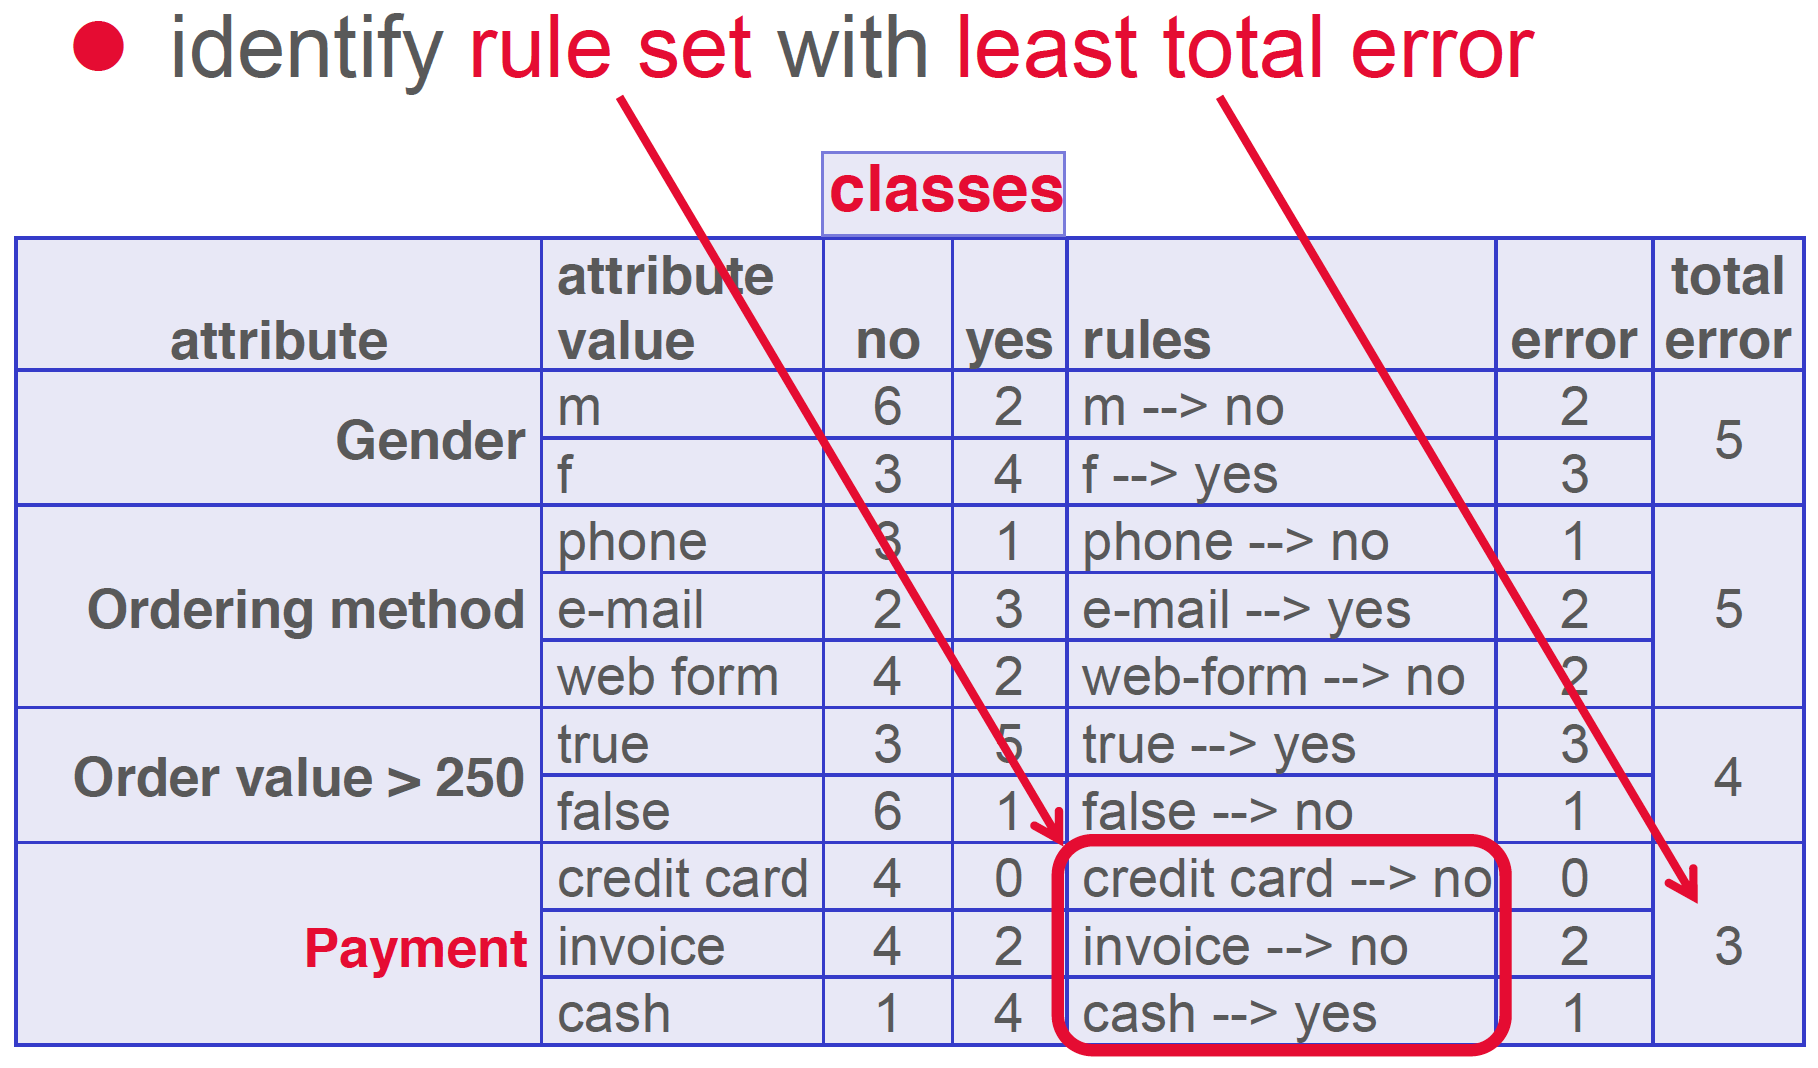
\includegraphics[width=.15\textwidth]{slides_images/1r_algorithm}
\end{center}
\end{breakbox}

\begin{breakbox}
\boxtitle{ID3-Algorithm:}
Used to create decision trees.
\begin{enumerate}
	\item Start with root node where no attribute is assigned yet. Root node contains full set of training instances.
	\item Identify individual classes and determine distribution of classes over instances.
	\item Calculate information content of current node (see below).
	\item Choose remaining attribute (not examined yet on path between current node of tree and root node). If no attributes left $\rightarrow$ exit.
	\item Determine attribute's value domain. Create preliminary child node for each distinct value.
	\item Partition set of instances (i.e. assign them to individual child nodes).
	\item Determine distribution of classes for each partition (child node).
	\item Calculate entropy of child nodes (see below).
	\item Calculate information gain (see below).
	\item If attributes left for examinig $\rightarrow$ go to 4.
	\item Select attribute with highest information gain. Insert it into current tree node. This attribute will not be considered any more in dependent sub-trees.
	\item Append attribute's child nodes to current tree node.
	\item Go to leftmost child node which is neither leaf nor has fully developed subtree structure. If there is none $\rightarrow$ go to next sibling node which is no leaf. If there is none either $\rightarrow$ go to parent node. If parent node is root node $\rightarrow$ exit, else repeat 13.
	\item Go to 4.
\end{enumerate}

\begin{breakbox}
\boxtitle{Calculate information content:}
\begin{align*}
info[s_1, ..., s_n]=\\
\frac{-\sum s_i log_2(s_i)+ \sum s_i log_2(\sum(s_i))}{\sum{s_i}}
\end{align*}
\end{breakbox}

\begin{breakbox}
\boxtitle{Calculate entropy:}
\begin{center}
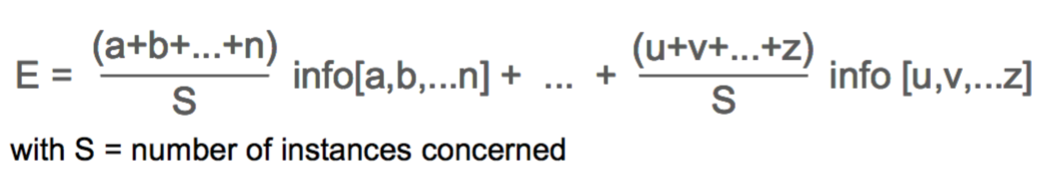
\includegraphics[width=.15\textwidth]{slides_images/entropy}
\end{center}
\end{breakbox}

\begin{breakbox}
\boxtitle{Calculate information gain:}
\newline Gain = info[parent node] - E[child node]
\end{breakbox}
\end{breakbox}

\begin{breakbox}
\boxtitle{Prepruning:}
\newline Stop construction before split is executed:
\begin{itemize}
	\item do not develop certain branches.
	\item nodes are set to leafs though not homogenous yet.
\end{itemize}
Executed during tree construction:
\begin{itemize}
	\item e.g.: information gain achieved by a certain split does not surmount a pre-defined threshold $\rightarrow$ split is omitted.
\end{itemize}
\end{breakbox}

\begin{breakbox}
\boxtitle{Postpruning:}
\begin{itemize}
	\item reverse splits
	\item execution after full development of tree
	\item merging of child nodes (e.g.: calculate the tree's error rate (incorrectly classified instances / all instances) if child nodes would be merged. If rate is below pre-defined threshold then merge (i.e. eliminate the sub-tree)).
\end{itemize}
\end{breakbox}

\begin{breakbox}
\boxtitle{C4.5} Another algorithm to create trees. Extension of
ID3.
\end{breakbox}

\begin{breakbox}
\boxtitle{Naïve Bayes:}
\begin{itemize}
	\item $P(C_i|X_i) = \frac{P(X_i|C_i)\cdot P(C_i)}{P(X_i)}$
	\item $P(X_i|C_i) =\\ \frac{\#\ Training\ instances\ of\ C_i\ with X_i}{\#\ Training instances\ of\ C_i}$
\end{itemize}
\end{breakbox}
